\documentclass{beamer}
\mode<presentation>
{
  \usetheme{Darmstadt}
  \definecolor{BYUBlue}{RGB}{00,22,55}
  \definecolor{BYUTan}{RGB}{232,211,175}
  \usecolortheme[named=BYUBlue]{structure}
  \setbeamercolor*{palette primary}{use=structure,fg=BYUBlue,bg=lightgray}
  \setbeamercolor*{palette quaternary}{fg=white,bg=lightgray!0!BYUBlue}
  \setbeamercolor{frametitle}{fg=BYUBlue,bg=BYUBlue!10}
  \setbeamertemplate{items}[circle]
  \setbeamertemplate{blocks}[rounded][shadow=True]
  \setbeamertemplate{navigations symbols}{circle}
}

\usepackage{graphics}
\usepackage[english]{babel}
\usepackage[utf8]{inputenc}
\usepackage{times}
\usepackage{forest}
\usepackage{subfigure}
\usepackage{caption}
\captionsetup{labelformat=empty}% redefines the caption setup of the figures environment in the beamer class.
\usepackage[T1]{fontenc}
\usepackage{array}
\usepackage{amsmath,amssymb}
\usepackage{booktabs}
\usepackage{colortbl}
\usepackage{array}
\usepackage{threeparttable}
\usepackage{multirow}
\usepackage{amsthm}
\usepackage{float,graphicx,color}
\usepackage{graphics}
\usepackage{multicol}
\usepackage{natbib}
\usepackage{color}
\usepackage{hyperref}
\hypersetup{colorlinks, urlcolor=blue}
\usepackage{threeparttable}
% \usepackage[format=hang,font=normalsize,labelfont=bf]{caption}
% \usepackage{subcaption}
\usepackage{delarray}
\usepackage{amssymb}
\usepackage{setspace}
\usepackage{placeins}
\usepackage{multirow}
\usepackage{mathtools}
\usepackage{animate}
\usepackage{bm}
\usepackage{amsmath,bm}
\usepackage{amssymb}
\usepackage{amsthm}
\newtheorem*{thm}{Theorem}
\theoremstyle{definition}
\newtheorem*{defn}{Definition}
\newcommand\ve{\varepsilon}
\newcommand\norm[1]{\left\lVert#1\right\rVert}
\DeclareMathOperator*{\argmin}{argmin}

% Python code blocks --------------------------------------
\usepackage{pythonhighlight}
\usepackage{tcolorbox}
\definecolor{codegreen}{rgb}{0,0.6,0}
\definecolor{codegray}{rgb}{0.5,0.5,0.5}
\definecolor{codepurple}{rgb}{0.58,0,0.82}
\definecolor{backcolour}{rgb}{0.95,0.95,0.92}

\lstdefinestyle{mystyle}{
    backgroundcolor=\color{backcolour},
    commentstyle=\color{codegreen},
    keywordstyle=\color{magenta},
    numberstyle=\tiny\color{codegray},
    stringstyle=\color{codepurple},
    basicstyle=\ttfamily\footnotesize,
    breakatwhitespace=false,
    breaklines=true,
    captionpos=b,
    keepspaces=true,
    numbers=left,
    numbersep=5pt,
    showspaces=false,
    showstringspaces=false,
    showtabs=false,
    tabsize=2
}

\lstset{style=mystyle}


\title[OG-PHL Input/Output]{OG-PHL: Input and Output}

\author[DeBacker and Evans]{\textbf{Jason DeBacker} \inst{1} \and \textbf{Richard W. Evans} \inst{2}}
\institute[shortinst]{\inst{1} University of South Carolina, Department of Economics \and
\inst{2} Abundance Institute, Open Research Group, Inc.}

\date[Short Occasion]{\textbf{January 15, 2026} \\ United Nations, Philippines}

\begin{document}

\begin{frame}
  \titlepage
\end{frame}


\section{Intro}

  \begin{frame}
    \frametitle{Overview}
    \begin{itemize}
      \item OG-PHL Inputs
      \begin{itemize}
        \item Parameters and larger objects
        \item Where to find them
      \end{itemize}
      \vspace{2mm}
      \item OG-PHL Output
      \begin{itemize}
        \item Where it is
        \item How to access it
        \item Different ways to display it
      \end{itemize}
      \vspace{2mm}
      \item Ways to run the model
    \end{itemize}
    \vspace{2mm}
    \begin{alertblock}{Takeaway}
      Basic understanding of model parameters, outputs, and how to run the model
    \end{alertblock}
  \end{frame}


\section{Inputs}

  \begin{frame}
    \frametitle{OG-PHL Inputs}
    \begin{block}{Two types of inputs}
      Parameters and arrays: Necessary info for model simulation
    \end{block}
    \vspace{2mm}
    \begin{itemize}
      \item New description of all parameters in OG-Core appendix chapter ``\href{https://pslmodels.github.io/OG-Core/content/intro/parameters.html}{Model parameters}''
      \vspace{2mm}
      \item New list of uniquely calibrated parameters in \href{https://eapd-drb.github.io/OG-PHL/content/calibration/exogenous_parameters.html}{OG-PHL documentation}
      \vspace{2mm}
      \item Best description in OG-Core \href{https://github.com/PSLmodels/OG-Core/blob/master/ogcore/default_parameters.json}{\texttt{default\_parameters.json}} file
      \vspace{2mm}
      \item Other inputs, such as demographics, are created/updated with other files like \href{https://github.com/PSLmodels/OG-Core/blob/master/ogcore/parameters.py}{\texttt{parameters.py}} in OG-Core, and \href{https://github.com/EAPD-DRB/OG-PHL/blob/main/ogeth/calibrate.py}{\texttt{calibrate.py}} in OG-PHL
    \end{itemize}
  \end{frame}

  \begin{frame}
    \frametitle{Default parameters and parameters object}
    \begin{itemize}
      \item Go through OG-Core \href{https://github.com/PSLmodels/OG-Core/blob/master/ogcore/default_parameters.json}{\texttt{default\_parameters.json}} and ``\href{https://pslmodels.github.io/OG-Core/content/intro/parameters.html}{Model parameters}'' chapter
      \vspace{3mm}
      \item Instantiate a default OG-Core parameters object in notebook
      \vspace{3mm}
      \item Go through OG-PHL \href{https://github.com/EAPD-DRB/OG-PHL/blob/main/ogeth/ogphl_default_parameters.json}{\texttt{ogphl\_default\_parameters.json}}
      \vspace{3mm}
      \item Update the parameters object in notebook to OG-PHL default
      \vspace{3mm}
      \item Show how to update and change parameters in scripts
    \end{itemize}
  \end{frame}


\section{Output}

  \begin{frame}
    \frametitle{OG-PHL output}
    \begin{columns}
      \begin{column}{0.5\textwidth}
        Two main output files for each Simulation
        \vspace{5mm}
        \begin{itemize}
          \item \texttt{SS\_vars.pkl}
          \vspace{5mm}
          \item \texttt{TPI\_vars.pkl}
        \end{itemize}
        \vspace{3mm}
        \begin{block}{Notebook}
          Go through output and image objects and show automatic functionality
        \end{block}
      \end{column}
      \begin{column}{0.5\textwidth}
        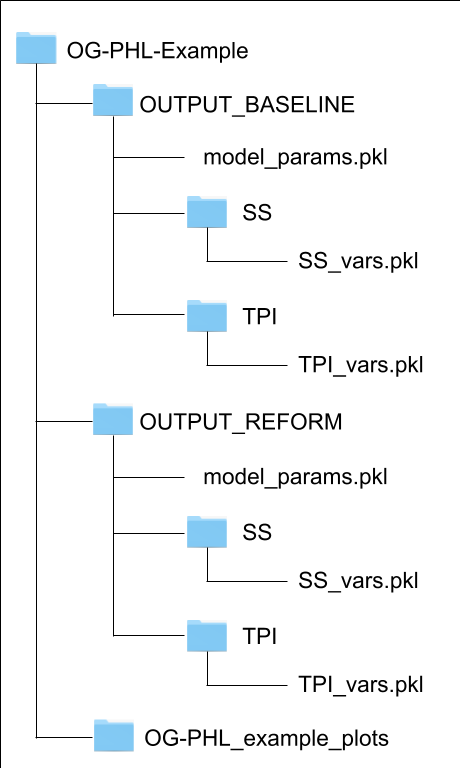
\includegraphics[width=0.75\textwidth]{./images/output_folders_phl.png} \\
      \end{column}
    \end{columns}
  \end{frame}


\section{Ways to run}

  \begin{frame}
    \frametitle{Ways to run OG-PHL}
    \begin{enumerate}
      \item (Local) Clone/download all repository files
      \begin{itemize}
        \item Best for developing and customizing
        \item Create \texttt{ogphl-dev} conda environment
        \item Run either with Python scripts or in Jupyter notebook
      \end{itemize}
      \vspace{4mm}
      \item (Local) \texttt{pip install ogphl} from PyPI.org
      \begin{itemize}
        \item Best if only want parameter changes, and don't need to change underlying model
        \item Run either with Python scripts or in Jupyter notebook
      \end{itemize}
      \vspace{4mm}
      \item (Cloud) Run in Google Colab using \texttt{pip install ogphl} (\href{https://tinyurl.com/ogphl-colab}{https://tinyurl.com/ogphl-colab})
    \end{enumerate}
  \end{frame}

  \begin{frame}
    \centering\LARGE\href{https://tinyurl.com/ogphl-colab}{https://tinyurl.com/ogphl-colab} \\
    \vspace{8mm}
    \centering
\includegraphics[width=0.5\textwidth]{./images/colab-qr-phl.png}
  \end{frame}

\end{document}
